\subsubsection{Description}

\begin{figure}[H]
	\centering
	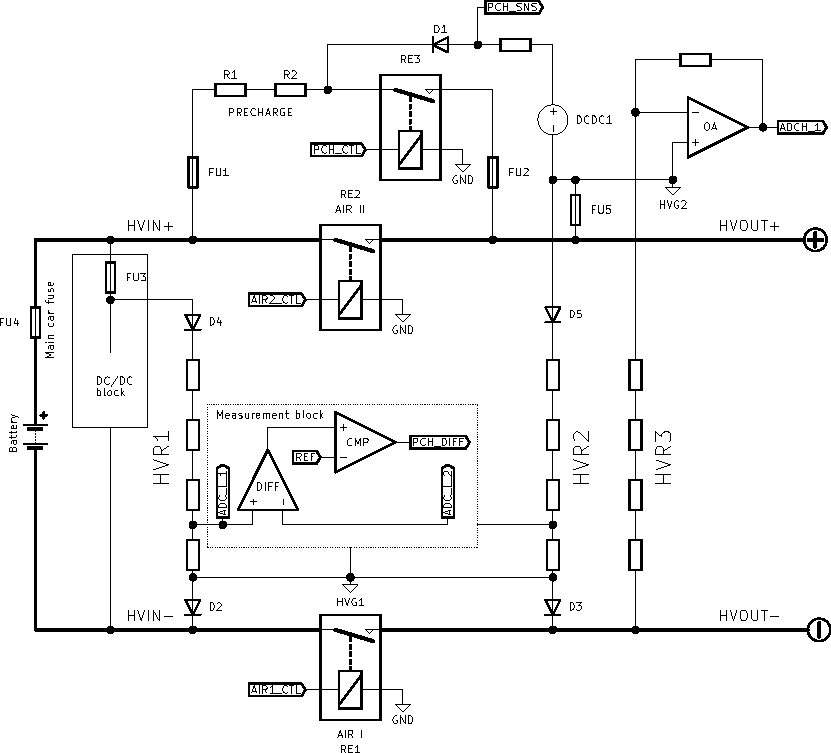
\includegraphics[width=\textwidth,clip]{./img/ECUA_AIRS.pdf}
	\caption{TS pre-charge circuit and switching schematic.}
	\label{fig:precharge_sch}
\end{figure}

Principial block schematic of the TS switching circuit (including pre-charge) is in the \ref{fig:precharge_sch}. Pre-charge circuit is part of and controlled by ECUA. Pre-charge circuit is comprised of a relay RE3 and two series connected power resistors R1 and R2. 

Both resistors are located on a heat-sink, that is shared with the DC/DC converters, mentioned in section 9.2 of this document. The task of the heat-sink is to enhance the power overload capacity of the pre-charge resistors during the initial overload during the beginning of the charging curve, shown in \ref{fig:precharge_voltage_time}.

\begin{figure}
	\begin{tikzpicture}
		\begin{axis}[
			use units,
			x unit=s,
			y unit=V,
			xlabel=time,
			ylabel=volatge,
			width=0.9\textwidth,
			height=0.5\textwidth,
			grid=major,
			xmin=0,
			ymin=0,
			xmax=10
			]
		\addplot[red, smooth] table[
			x=time,
			y=voltage,
			col sep=comma
			] {./data/TS_precharge.csv};
		\end{axis}
		\end{tikzpicture}
		\caption{Pre-charge voltage in time.}
	\label{fig:precharge_voltage_time}
\end{figure}

The formula describing \ref{fig:precharge_voltage_time} is:

\begin{equation}
	I_{d}=1-e^{(\frac{-t}{R*C})}
	\label{eq:precharge_voltage}
\end{equation}

\begin{figure}
	\begin{tikzpicture}
	\begin{axis}[
	use units,
	x unit=s,
	y unit=A,
	xlabel=time,
	ylabel=current,
	width=0.9\textwidth,
	height=0.5\textwidth,
	grid=major,
	xmin=0,
	ymin=0,
	xmax=10
	]
	\addplot[red, smooth] table[
	x=time,
	y=current,
	col sep=comma
	] {./data/TS_precharge.csv}; 
	\end{axis}
	\end{tikzpicture}
	\caption{Precharge current in time.}
	\label{fig:precharge_current_time}
\end{figure}


The formula describing \ref{fig:precharge_current_time} is:

\begin{equation}
	I_{d}=\frac{V_{c}}{R_{d}}	
\end{equation}

\begin{equation}
	I_{d}=\frac{V_{s}*(1-e^{(\frac{-t}{R*C})})}{R_{d}}
	\label{eq:precharge_current}
\end{equation}


Both wirewound power resistors, ARCOL HS25 series, have 250 $\Omega$, 25 W continuous rating, DATASHEET.

All three TS relays RE$_1$ to RE$_3$ coils are powered directly from the SDC end.

After the SDC circuit is complete and closed (voltage present at SDC END), the precharge sequence is begun by closing AIR I (RE1). Then a pre-charge relay RE3 is closed. Voltage both on the ACP and output side is monitored using the measurement block, through the $HVR_1$ and HVR$_2$ resistor dividers. After the voltage difference is low enough (determined by ECUA software), AIR II (RE2) is closed, RE3 can be released.

Safety of the AIR switching and pre-charging is done by the ECUA firmware, that evaluates all possible circuit states. Voltages are measured on the ACP and ACP output sides using the measurement block, AIR physical states are observed using the auxiliary contacts and the pre-charge relay physical contact state is observed using the principle in the \ref{fig:precharge_sch}, via the diode D$_1$. The PCH\_SNS signal is pulled low whenever the pre-charge relay RE3 contact is closed.

Several safety precautions are implemented, on top of the Rules. First of such implemented protections is HW non-programmable voltage difference sensing across the pre-charge relay or AIR II respectively. This is done using the two voltage measurement dividers HVR$_1$ and HVR$_2$. There is a differential amplifier and comparator, that prevents closing both AIR relays in case of high voltage difference across the AIR II. 

Diodes D2 and D3 serve to block current flow to the output in case of AIR I is open. This specific topology was chosen to be able to measure the difference voltage across the AIR II utilizing only analog non-programmable circuitry.

Second precaution is a HW circuit limiting the maximum pre-charge relay closed time, and assuring a minimum off time for the pre-charge resistor to cool off. This circuit is a non-programmable one, realized using a discrete logic. In case of a pre-charge time-out or failure (voltages not equalized), AIR I (the Tyco Kilovac EV200 ODKAZNAKONECUZJETAMDATASHEET) is disconnected always first (instead of the pre-charge relay RE3), because the AIR does have the required DC breaking capacity.

Additional precision ACP voltage measurement is taken using the HVR$_3$ sense divider, as this measurement is not influenced by the forward voltage drops of diodes D$_2$ to D$_5$. This measurement together with the measured ACP current serves to calculate power drawn from the ACP. This measurement is then presented on the CAN bus for other car ECUs, for example to estimate the SOC, instantenous power, etc.  

The TS voltage sensing dividers HVR1, HVR2 and HVR3 are realized with a high voltage 3500 V rated resistors from Vishay, HVR37 series (DATASHEEEEET). All dividers use 10 Mohm resistors as the top side of the divider. All diodes D1 to D5 are SM4007 (DATASHEET) or equivalent type, 1000 V rated. The blocking voltage is therefore sufficient to safely withstand the maximum ACP voltage of 400 V.

\paragraph{Pre-charge safety on ECUA}
Except from what rules require we implemented several safety precautions. In case, that SDC error doesn’t occur and driver pushed TS ON button following safety precautions are taken to prevent switching AIR in case of problem that has not yet been detected.

First one is completely non-programmable protection against switching voltage difference by AIR. It uses voltage measurement and then comparators and logic to disable microcontroller decision in case of SW error.
Second one is measuring all states and voltages by microcontroller on ECUA which can determinate error before non-programmable protection would have to act.

Third (time-out) protection is used when everything seems to be OK, but the charging is too slow – caused by too high pre-charge resistance (any of pre-charge resistors fails), or some leakage of charge in capacitor or any other possible error occurs. If voltage difference is not equaled in time less them 2seconds, the ECUA stops pre-charge and waits 5 seconds before trying again. (In order to not overpower resistors.) If number of attempts to pre-charge is in this state higher then 8, something is clearly wrong and ECUA opens SDC and indicates error. Sending message about error and sets car into not-ready state.

\subsubsection{Wiring, cables, current calculations, connectors}
Describe wiring, show schematics, describe connectors and cables used and show useful data regarding the wiring.

%\item Give a plot “Percentage of Maximum Voltage” vs. time
%\item Give a plot Current vs. time 
%\item For each plot, give the basic formula describing the plots


Additionally, fill out the tables:

\begin{table}[H]
	\centering
	\caption{General data of the pre-charge resistor}
	\begin{tabularx}{\textwidth}{|X|X|}
		\hline
		Resistor Type: & \\[\TableSize]
		\hline
		Resistance: & \\[\TableSize]
		\hline
		Continuous power rating: & \\[\TableSize]
		\hline
		Overload power rating (1 sec): &  \\[\TableSize]
		\hline
		Overload power rating (5 sec): &  \\[\TableSize]
		\hline
		Overload power rating (15 sec): &  \\[\TableSize]
		\hline
		Voltage rating: & \\[\TableSize]
		\hline
		Cross-sectional area of the wire used: & \\[\TableSize]
		\hline
	\end{tabularx}%
	\label{tab:precharge-general}%
\end{table}%

\begin{table}[H]
	\centering
	\caption{General data of the pre-charge relay}
	\begin{tabularx}{\textwidth}{|X|X|}
		\hline
		Relay Type: & \\[\TableSize]
		\hline
		Contact arrangment: &  \\[\TableSize]
		\hline
		Continuous DC current:  & \\[\TableSize]
		\hline
		Voltage rating  & \\[\TableSize]
		\hline
		Nominal Coil Voltage: &  \\[\TableSize]
		\hline
		FET type: &  \\[\TableSize]
		\hline
		Maximum Drain-Source Current: &  \\[\TableSize]
		\hline
		Drain-Source Breakdown Voltage: &  \\[\TableSize]
		\hline
		On Charasteristics Gate Threshold Voltage: & \\[\TableSize]
		\hline
		Cross-sectional area of the wire used: & \\[\TableSize]
		\hline
	\end{tabularx}%
	\label{tab:precharge-relay}%
\end{table}%

\subsubsection{Position in car}
%Provide CAD-renderings showing all relevant parts. Mark the parts in the rendering, if necessary.

\begin{figure}[H]
	\centering
	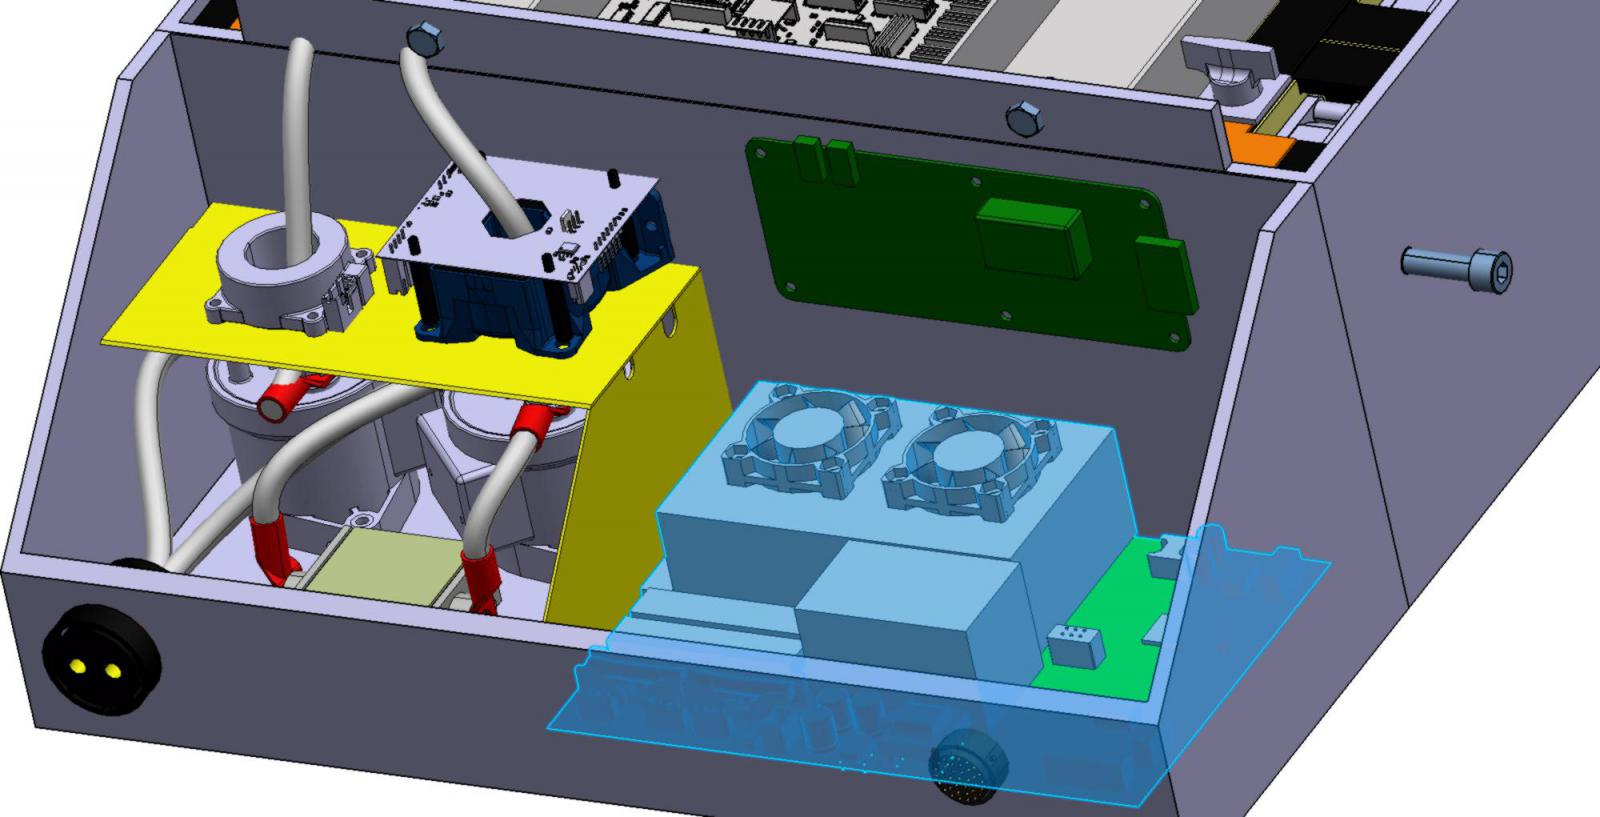
\includegraphics[width=\textwidth]{./img/ECUA_POSITION.jpg}
	\caption{ECUA position.}
	\label{fig:ECUA}
\end{figure}